\documentclass[12pt]{article}
\usepackage{amsmath}
\usepackage[lmargin = 1in, rmargin = 1in, tmargin = 1in, bmargin = 1in]{geometry}
\usepackage[none]{hyphenat}
\usepackage{graphicx}
\usepackage{subcaption}
\usepackage{float}

\title{\textbf{Problem 2\\Neural Network Implementation}}
\author{Aditya Vipradas\\ASU ID: 1209435588}
\begin{document}
\maketitle
The given data of 250 samples is fed to the inbuilt neural network toolbox in MATLAB. Default 10 hidden layers are used. Samples used for training, test and validation are 70, 15 and 15 respectively. The neural network flow diagram is as follows.
\begin{figure}[H]
\begin{center}
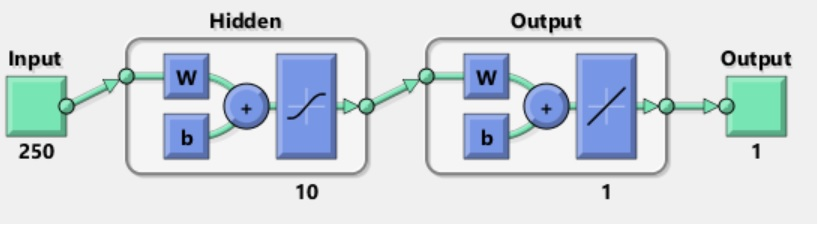
\includegraphics[scale=0.4]{nn0.jpg}
\caption{Neural network flow diagram}  
\end{center}
\end{figure}
The performance charts obtained are as follows. As seen in the following plot, best validation is obtained at epoch 6.
\begin{figure}[H]
\begin{center}
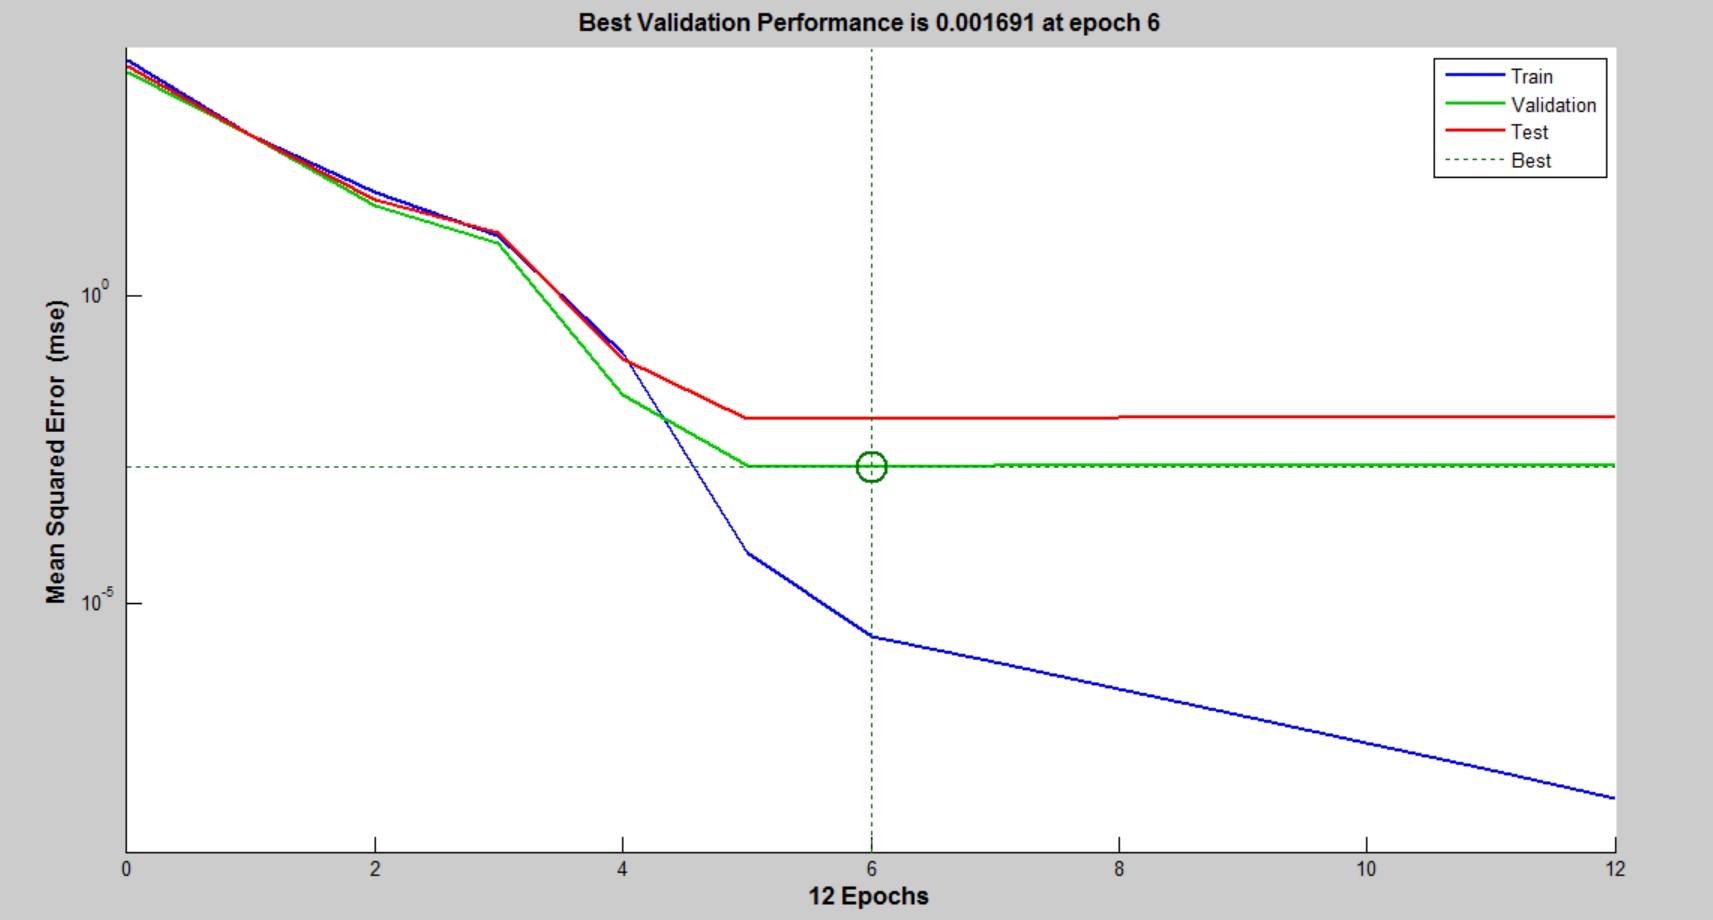
\includegraphics[scale=0.4]{nn1.jpg}
\caption{Performance plot}  
\end{center}
\end{figure}
\begin{figure}[H]
\begin{center}
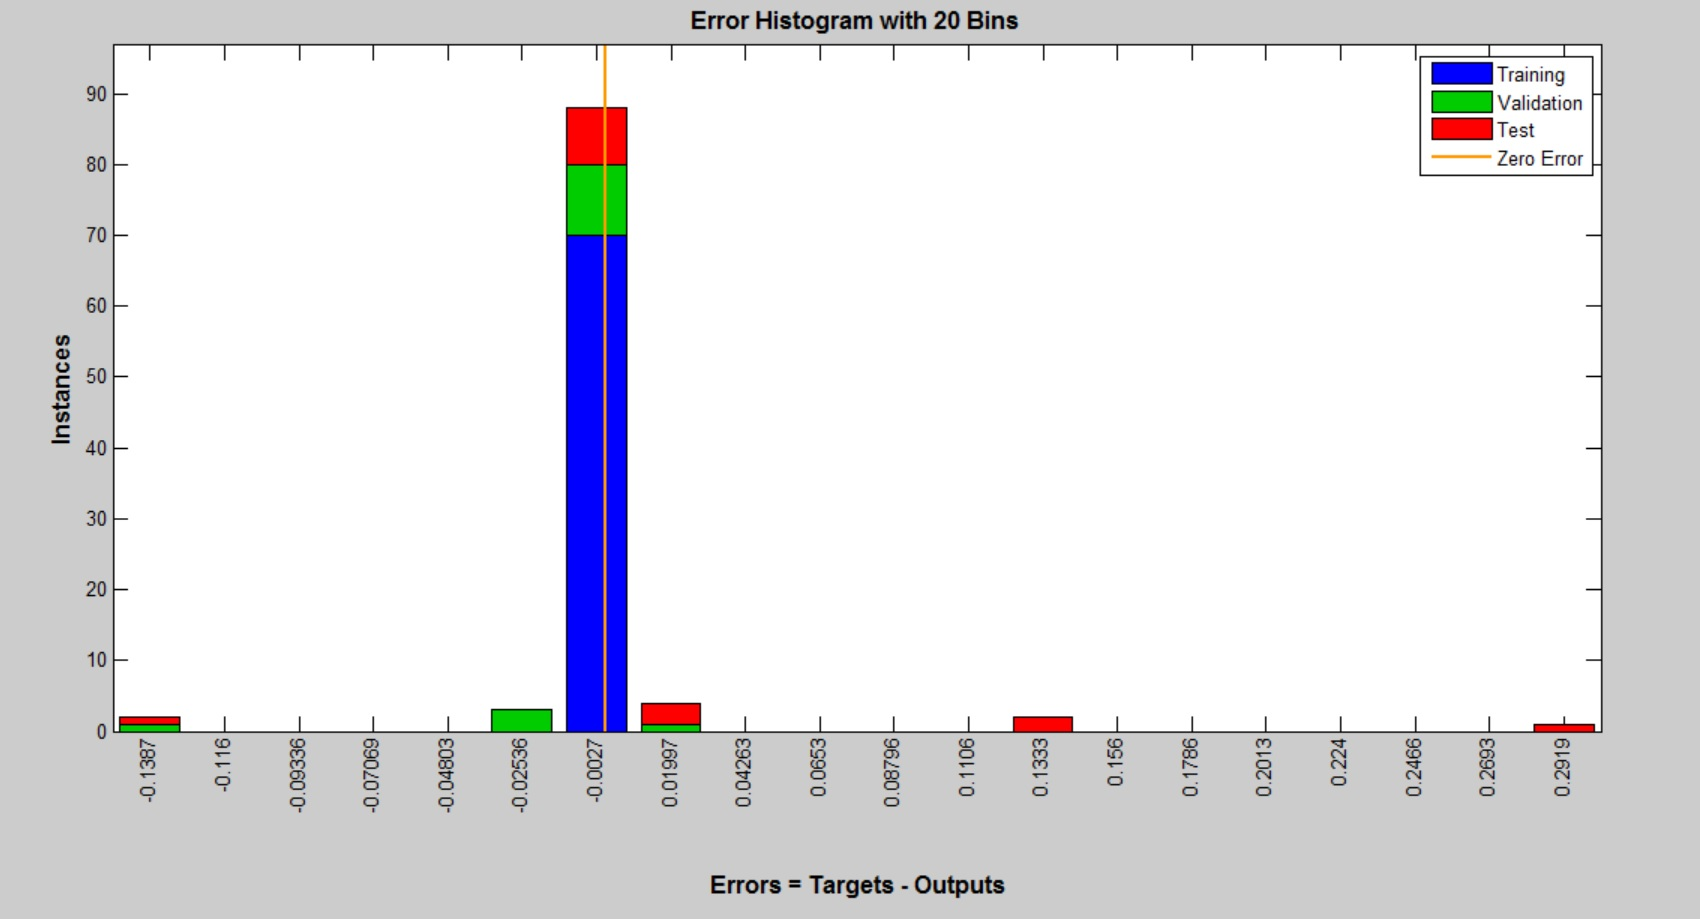
\includegraphics[scale=0.4]{nn2.jpg}
\caption{Error Histogram}  
\end{center}
\end{figure}
\begin{figure}[H]
\begin{center}
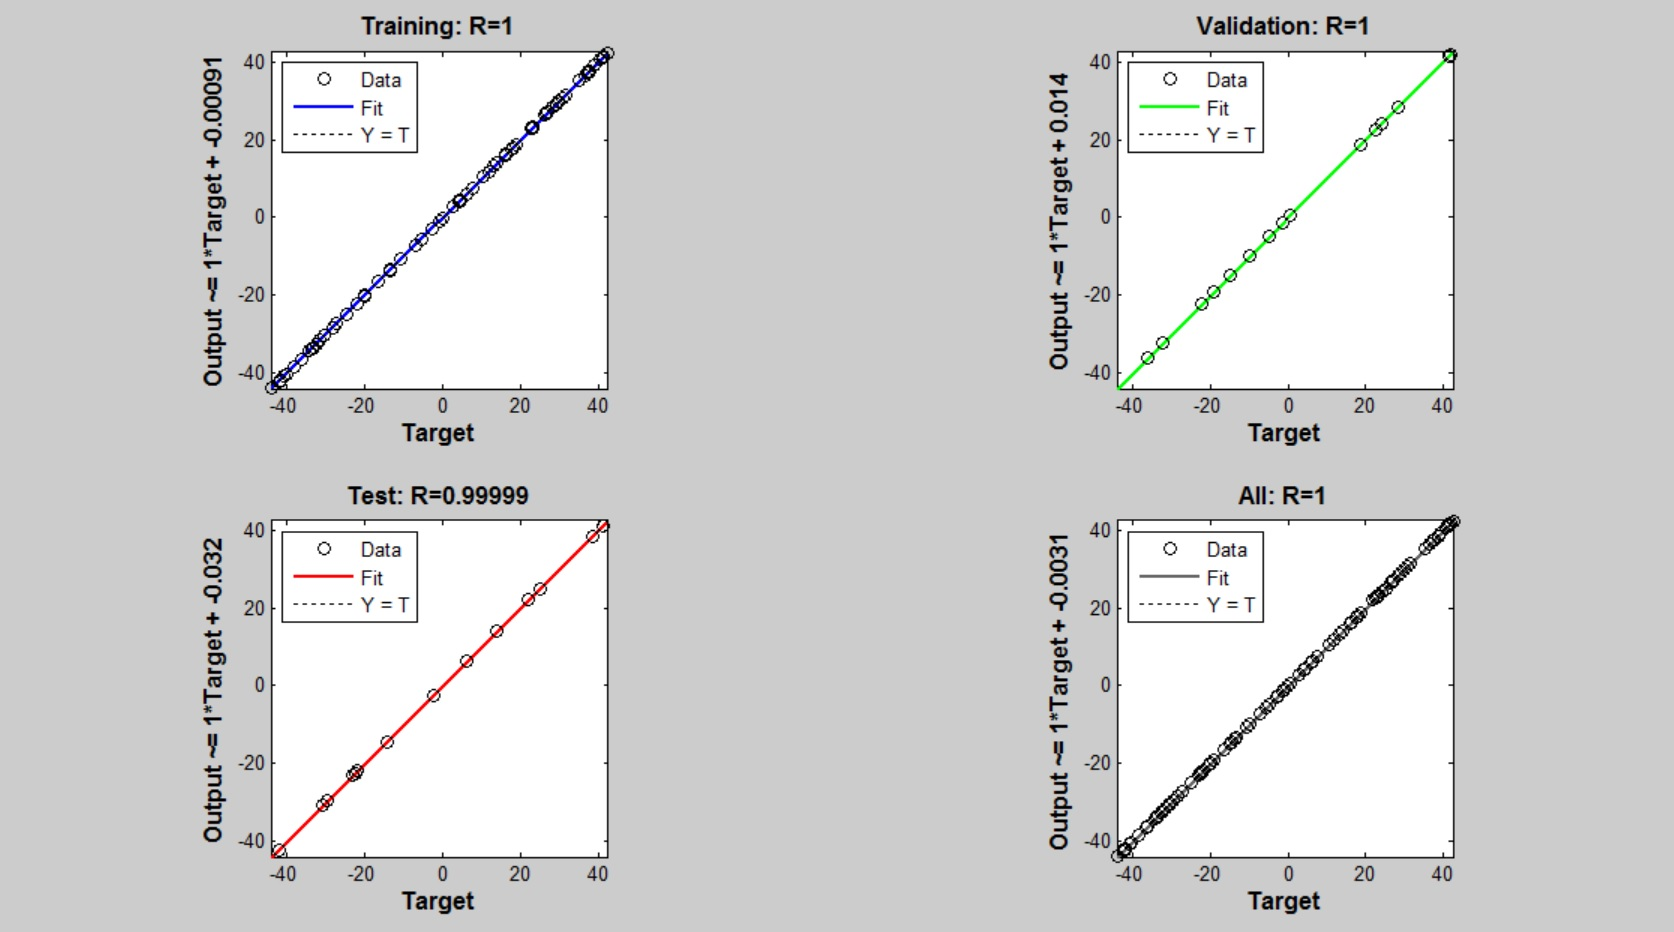
\includegraphics[scale=0.4]{nn3.jpg}
\caption{Regression Plot}  
\end{center}
\end{figure}
As seen from the regression plot, the R value measure for all the outputs is 1. This suggests that the curve fit to the given data is acceptable.
\begin{figure}[H]
\begin{center}
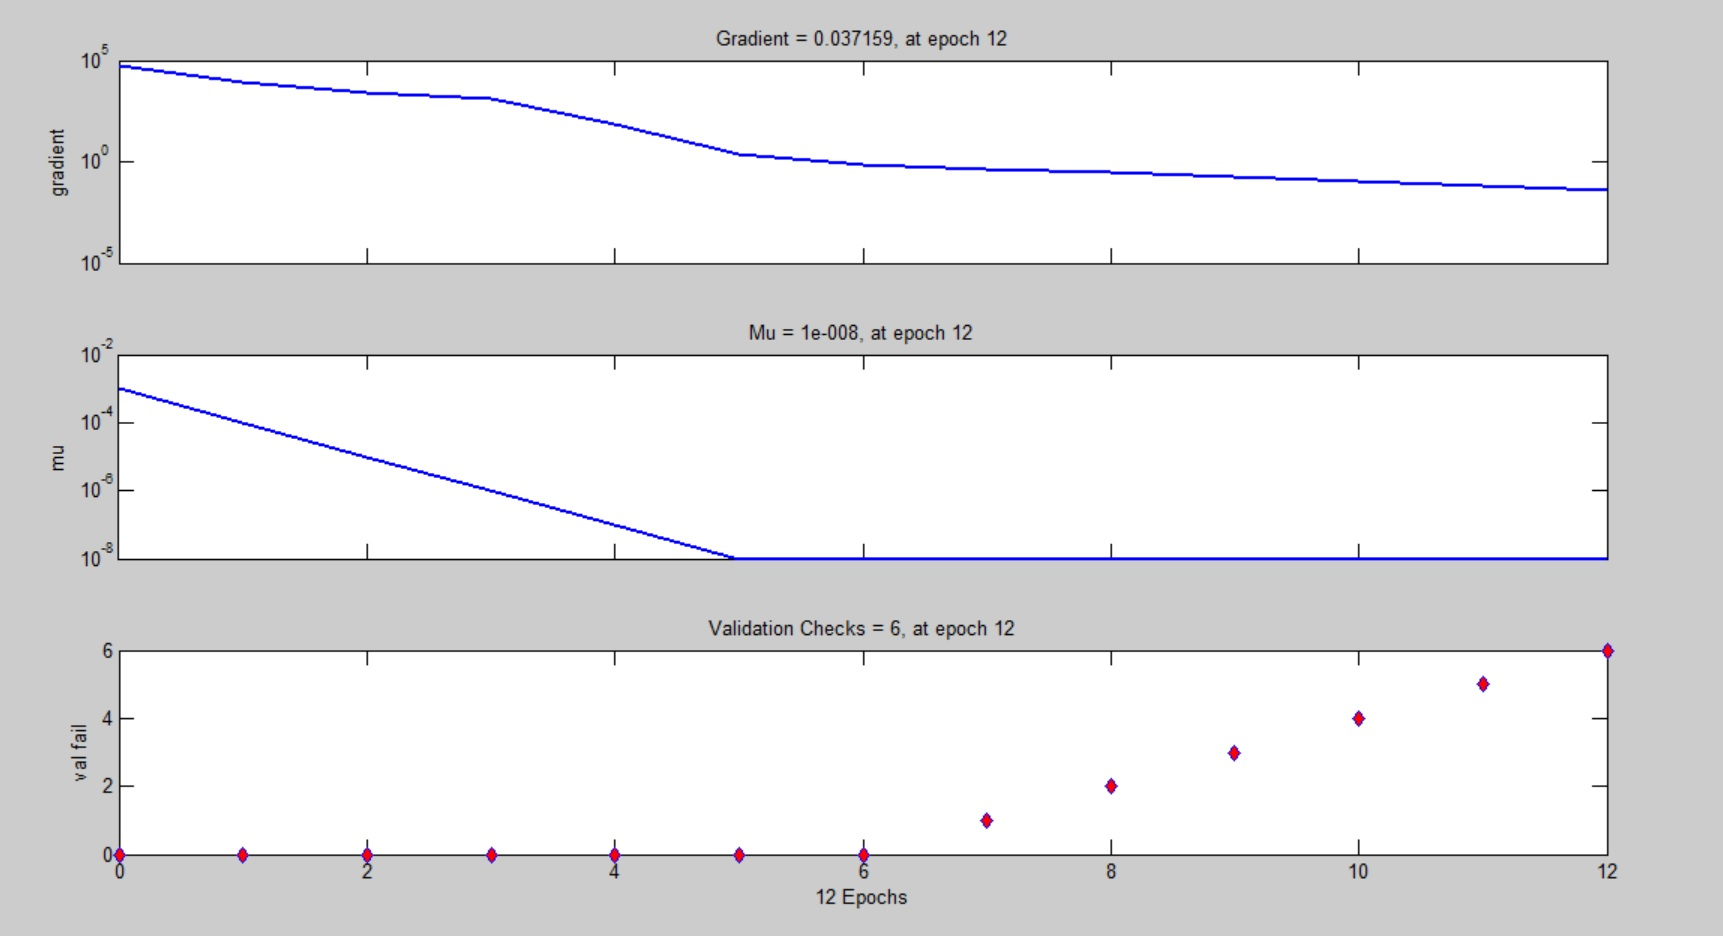
\includegraphics[scale=0.4]{nn4.jpg}
\caption{Training state plot}  
\end{center}
\end{figure}
This is the test performance report for the neural network (Levenberg-Marquardt training) implementation on the given non-linear data set.
\end{document}